\documentclass[11pt,a4paper]{article}
\usepackage{amsmath,amsfonts,amssymb,amsthm,epsfig,epstopdf,url,array,graphicx,xspace}
\usepackage[english]{babel}


\theoremstyle{plain}
\newtheorem{thm}{Theorem}[section]
\newtheorem{lem}[thm]{Lemma}
\newtheorem{fact}{Fact}[section]
\newtheorem{assm}{Assumption}[section]
\newtheorem*{assm*}{Assumption}
\newtheorem{prop}[thm]{Proposition}
\newtheorem*{cor}{Corollary}

\theoremstyle{definition}
\newtheorem{defn}{Definition}[section]
\newtheorem{conj}{Conjecture}[section]
\newtheorem{exmp}{Example}[section]

\theoremstyle{remark}
\newtheorem*{rem}{Remark}
\newtheorem*{note}{Note}

\newcommand{\ie}{i.e.\@\xspace}
\newcommand{\eg}{e.g.\@\xspace}

\renewcommand{\emptyset}{\ensuremath{\varnothing}}
%\newcommand{\makeintoafunction}[1]{\textsc{#1}}
\newcommand{\makeintoafunction}[1]{\textit{\uppercase{\small #1}}}
\newcommand{\APPLY}{\makeintoafunction{apply}}
\newcommand{\SAFE}{\makeintoafunction{safe}}
\newcommand{\AFFECTED}{\makeintoafunction{affected}}
\newcommand{\OBSERVED}{\makeintoafunction{observed}}
\newcommand{\AREA}{\makeintoafunction{area}}
\newcommand{\VALIDATORS}{\makeintoafunction{validators}}
\newcommand{\PARENT}{\makeintoafunction{parent}}
\newcommand{\SAMPLE}{\makeintoafunction{sample}}
\newcommand{\ANC}{\makeintoafunction{ancestor}}
\newcommand{\GET}{\makeintoafunction{get}}
\newcommand{\PGE}{\makeintoafunction{pge}}
\newcommand{\GDC}{\makeintoafunction{gdc}}
\newcommand{\PE}{\makeintoafunction{pe}}

\begin{document}


\title{Notes on Scalable Blockchain Protocols (version 0.3.1)}
\date{April 14-31, 2015}
\author{Vitalik Buterin (Ethereum) \\  \\ Reviewers and collaborators: Gavin Wood, Vlad Zamfir (Ethereum), \\ Jeff Coleman (Kryptokit)}

\maketitle

\begin{abstract}
We propose a technique for achieving scalable blockchain consensus by means of a ``sample-and-fallback'' game: split transactions up into collations affecting small portions of the blockchain state, and require that in order for a collation of transactions to be valid, it must be approved by a randomly selected fixed-size sample taken from a large validator pool. In case a bad collation does pass through employ a mechanism by which a node can ``challenge'' an invalid collation and escalate the decision to a much larger set of validators. Our scheme is designed as a generalized overlay that can be applied to any underlying blockchain consensus algorithm (\eg proof of work, proof of stake, social-network consensus) and almost any state transition function, provided that state changes are sufficiently ``localized''. Our basic designs allow for a network with nodes bounded by $O(N)$ computational power to process a transaction load and state size of $O(N^{2-\epsilon})$, though we also propose an experimental ``stacking'' strategy for achieving arbitrary scalability guarantees up to a maximum of $O(exp(N/k))$ transactional load.
\end{abstract}

\section{Introduction}

Currently, all blockchain consensus protocols that are actively in use have an important limitation: every fully participating node in the network must process every transaction. Although this requirement ensures a very strong guarantee of security, making it all but impossible for an attacker even with control over every node participating in the consensus process to convince the network of the validity of an invalid transaction, it comes at a heavy cost: every blockchain protocol that works in this way is forced to choose between limiting itself to a low maximum transaction throughput, with a resulting high per-transaction cost, and allowing a high degree of centralization.

What might perhaps seem like a natural solution, splitting the relevant data over a thousand blockchains, has the two fundamental problems that it (i) decreases security, to the point where the security of \emph{each individual blockchain} on average does not grow \emph{at all} as total usage \emph{of the ecosystem} increases, and (ii) massively reduces the potential for interoperability.

There are techniques, such that the practice of having proof-of-work miners mine multiple blockchains simultaneously (``merge-mining''), that seem to have stronger security, but in practice they end up offering at best a linear tradeoff between the thousand-chains and single-chain extreme: if each chain is mined by only one in a thousand miners, then it is vulnerable to very cheap attacks\cite{mmpetertodd} (and indeed, such attacks have been succesfully carried out in real life\cite{coiledcoin}), and if each chain is mined by every miner then every consensus participant must process every transaction anyway and so we have not made any progress in scalability. Techniques involving ``checkpointing'' a smaller blockchain inside a larger one also fail to provide security, as they do not prevent an attacker with majority participation in the smaller blockchain's consensus process from creating a checkpoint of fake or unavailable data.\cite{factompetertodd}

The problem of simulatenously achieving the best of both worlds: having only a small portion of consensus participants \emph{explicitly} participate in validating each transaction, but have the entire weight of the network \emph{implicitly} stand behind each one, has proven surprisingly hard.

There are several reasons why this is the case. First, because we lose the guarantee that a node can personally validate every transaction in a block, nodes must now necessarily employ statistical and economic means in order to make sure that other blocks are secure; in essence, every node can only \emph{fully} keep track of at most a few parts of the entire "state", and must therefore be a "light client", downloading only a small amount of header data and not performing full verification checks, everywhere else. However, even still that node's economic resources must somehow be involved in ``attesting'' to the security of all transactions, including those that it does not even know about.

Second, we need to be concerned not only with validity but also with data availability; it is entirely possible for a block to appear that looks valid, and is valid, but for which the auxiliary data is unavailable, leading to a situation where no other validator can effectively validate transactions or produce new blocks since the necessary data is unavailable to them. Finally, transactions must necessarily be processed by different nodes in parallel, and given that it is not possible to parallelize arbitrary computation \cite{parallelcomputing}, we must determine the set of restrictions to a state transition function that will best balance parallelizability and utility.

This paper proposes another strategy for achieving scalability, as well as some formalisms that can be used when discussing and comparing scalable blockchain protocols. The strategy revolves around splitting transactions up into ``collations'' which affect a particular portion of the blockchain state, and then using a ``sample-and-fallback'' game to validate the headers of individual collations: in order for any particular collation to be valid, require it to be approved by a randomly selected sample of validators, and in case a bad collation does come through employ a mechanism in which a node can challenge invalid collations, reverting the harmful transactions and transferring the malfeasant validators' security deposit to the challengers as a reward unless the challenge is answered by a confirmation of validity from a much greater number of validators.

Theoretically, under a Byzantine-fault-tolerant model of security, fallback is unnecessary; sampling only is sufficient. However, if we are operating in an anonymous-validator environment, then it is also considered desirable to have a hard economic guarantee of the minimum quantity of funds that needs to be destroyed in order to cause a certain level of damage to the network; in that case, in order to make the economic argument work we use fallback as a sort of incentivizer-of-last-resort, making cooperation the only subgame-perfect equilibrium.

The particular advantage that our designs provide is a very high degree of generalization and abstraction. Although schemes using technologies like auditable computation through Merkle-tree computation traces\cite{versum} and micropayment channels\cite{lightning} exist for increasing efficiency in specific use cases like processing complex verifications and implementing currencies, our designs can be used to provide scalability for any underlying state transition function, provided that most state changes have a ``localized'' impact. Our designs are also meant to be consensus-neutral, working equally well with proof of work, Tendermint-style\cite{tendermint} proof of stake, and even social-network consensus algorithms such the Stellar Consensus Protocol\cite{stellar} and Houwu Chen's simulated annealing algorithm\cite{chenhouwu}. Generality is achieved by splitting consensus into two levels, where the top-level consensus participants implement a state transition function that deals with root hashes of portions of the state and collation headers, while the bottom-level activity is involved in actually checking the validity of the underlying transactions.

Our basic designs allow for a network consisting solely of nodes bounded by $O(N)$ computational power to process a transaction load of $O(N^{2-\epsilon})$ (we generally use $O(N^\epsilon)$ to denote polylogarithmic terms for simplicity), under both Byzantine-fault-tolerant and economic security models; we then also propose an experimental ``stacking'' strategy for achieving arbitrary scalability guarantees up to a maximum of $O(exp(N/k))$ transactional load, although we recommend that for simplicity implementers attempt to perfect the $O(N^{2-\epsilon})$ designs first.

\section{Concepts and Definitions}

In order to facilitate the highly abstract discussion that is involved in our solution, we will start off by defining some basic terminology and creating a semi-formal language that can be used to deal with the mechanics of state transition functions in a highly abstract way. We will introduce \emph{cryptoeconomic state machines} as a formalism, and we will provide Bitcoin as an example, defining the \emph{state transition function}, \emph{consensus algorithm} and \emph{fork choice rule} involved, as well as describing several other projects so as to illustrate how one might change each individual component.

\begin{defn}[State]
A \emph{state} is the set of all stored information in a paticular system or application. For our purposes, the state will often include account balances, domain registrations, the code and data associated with on-chain objects such as smart contracts, etc.
\end{defn}

\begin{defn}[Transaction]
A \emph{transaction} is a piece of data representing an operation that a particular user wants to carry out. A transaction typically includes a cryptographic signature from which one can verify its sender.
\end{defn}

\begin{defn}[State Transition Function]
A \emph{state transition function} is a function $\APPLY(\sigma, \tau) \rightarrow \sigma'$, which takes as input a ``prior state'' (or ``pre-state'') $\sigma$ and a transaction $\tau$ and outputs the ``post-state'' $\sigma'$. If $\tau$ is ``invalid'' in the context of $\sigma$ in the intuitive sense (eg. $\sigma$ has account $A$ having a zero currency balabce and $\tau$ tries to send twenty currency units from $A$ to $B$), we conventionally say that $\sigma' = \varnothing$. We require that $\APPLY(\varnothing, \tau) = \varnothing$ for any $\tau$.
\end{defn}

For simplicity, we will use the following notation throughout:

\begin{itemize}
\item
$\APPLY(\sigma, \tau) = \sigma'$ becomes $\sigma + \tau = \sigma'$
\item  
Given an ordered list $T = [\tau_1, \tau_2, \tau_3...]$ and a state $\sigma$, we define $\sigma + T = \sigma + \tau_1 + \tau_2 + ...$
\item
$T = [\tau_1, \tau_2, \tau_3 ...]$ is \emph{valid in the context of $\sigma$} if $\tau_1$ is valid in the context of $\sigma$, $\tau_2$ is valid in the context of $\sigma + \tau_1$, $\tau_3$ is valid in the context of $\sigma + \tau_1 + \tau_2$, etc.
\item
$[n]$ is the set $\{1, 2, 3..... n\}$, as is standard in combinatorics.
\end{itemize}

We can describe a simplified Bitcoin-like cryptocurrency as follows:

\begin{itemize}
\item
The \emph{state} consists of a mapping $\mathcal{P} \rightarrow [0, \infty)$, where $\mathcal{P}$ is a set of public keys of users and the values are balances.
\item
A \emph{transaction} is a tuple $\tau = (from, to, value, sig)$, where $from$ is the sender public key, $to$ is the destination public key, $value$ is the amount that the transaction is sending and $sig$ is a cryptographic signature.
\item
A transaction $\tau = (from, to, value, sig)$ is valid in the context of a state $\sigma$ if all of the following hold true:
    \begin{itemize}
    \item
    $\sigma[from] \ge value$ (you can't spend more money than you have)
    \item
    $value \ge 0$
    \item
    $V(from, sig) = 1$ for some cryptographic verification function $V$ (\ie the signature is valid when verified against the sender public key, so you can't spend an account's money unless you have the corresponding private key)
    \end{itemize}
If $\tau$ is invalid, then $\sigma + \tau = \varnothing$. If $\tau$ is valid, then $\sigma + \tau$ is identical to $\sigma$ except:
    \begin{itemize}
    \item
    $\sigma'[from] = \sigma[from] - value$
    \item
    $\sigma'[to] = \sigma[to] + value$
    \end{itemize}
\end{itemize}

In reality, Bitcoin is somewhat more complicated, using a concept of \emph{unspent transaction outputs} to record the ownership of funds instead of a direct mapping of public keys to balances, but the above example illustrates the basic principle.

\begin{defn}[Block]
A \emph{block} $\beta$ is a package containing a list of transactions $T$, a reference to a \emph{parent block} (in more exotic protocols, blocks with multiple parents are sometimes found, but usually blocks only have one parent), and auxiliary verification data. A block is valid in the context of a state $\sigma$ if:
\begin{itemize}
\item
The block's transaction list is valid in the context of $\sigma$
\item
Some other conditions, generally determined by the consensus algorithm, are met.
\end{itemize}
If a block is valid, we define the block-level state transition function with $\sigma + \beta = \sigma + T$ (ie. $\sigma + \tau_1 + \tau_2 + ... + \tau_n$) where $T = [\tau_1, \tau_2 ... \tau_n]$ is the transaction list in $\beta$. If a block is invalid, then we once again conventionally specify $\sigma + \beta = \varnothing$. Note that the consensus algorithm will sometimes specify operations that are illegal in normal transactions; for example, Bitcoin specifies that the first transaction in a block can include an \emph{ex nihilo} reward of 25 BTC to the producer of that block, and Ethereum performs a similar operation at the end; although in Ethereum's case the rewarding step is performed directly by the protocol and not by an actual transaction, we can still consider it a kind of ``virtual transaction'' for our purposes.
\end{defn}

\begin{defn}[Blockchain]
A \emph{blockchain} is a tuple $(G, B)$ where $G$ is a \emph{genesis state} and $B = [\beta_1, \beta_2, \beta_3 ...]$ is an ordered list of blocks. A blockchain is \emph{valid} if every $\beta \in B$ is valid, and so $G + \beta_0 + \beta_1 + ... = \sigma_f$ is a valid state (\ie not $\varnothing$).
\end{defn}

\begin{defn}[Consensus algorithm]
A \emph{consensus algorithm} is an ensemble of two processes:
\begin{itemize}
\item
A \emph{fork choice rule}, a process which can be run by any node in order to determine what the current ``main chain'' is. Note that the fork choice rule also implicitly provides $\sigma_f$, the final state after sequentially processing all blocks.
\item
An \emph{updating process}, a process that is collectively performed by the participants in a network in order to produce a new block to extend the main chain.
\end{itemize}
\end{defn}

The consensus algorithm will in most cases specify additional block validity conditions. In the case of Bitcoin, the consensus algorithm is known as ``proof of work'', and the parts can be summarized as follows:

\begin{itemize}
\item
The \emph{updating process} consists of thousands of nodes around the world repeatedly attempting to produce blocks with powerful computers until some node finds one satisfying $sha256(\beta) < \frac{2^{256}}{D}$, where $D$ is a difficulty parameter that updates so as to ensure that a block is produced on average every ten minutes. Because $sha256$ is a pseudorandom hash function, there is no way to produce a valid block that is faster than simply trying different modifications to the block data until you eventually produce a block that passes, and this process on average collectively takes the whole network $D$ iterations.
\item
The \emph{fork choice rule} consists of choosing the blockchain that has the highest \emph{total difficulty}, \ie the greatest amount of statistically expected computational work placed into building the whole chain.
\item
The additional \emph{block validity conditions} are:
    \begin{itemize}
    \item
    $sha256(\beta) \le \frac{2^{256}}{D}$
    \item
    The first transaction is allowed to create an \emph{ex nihilo} reward of 25 BTC to the producer of the block
    \end{itemize}
\end{itemize}

Note that in this case, the updating process and the block validity conditions are the same, but this is not always the case; for example, in Tendermint\cite{tendermint}, the validity condition is simply that a block must be signed by two thirds of a pool of validators, but a traditional Byzantine-fault-tolerant consensus algorithm is used in the consensus process to facilitate agreement on which block validators should sign.

\begin{defn}[Weight function]
A \emph{weight function} is a mapping $U \rightarrow x \in [0,1]$ where $U$ is a user, such that the sum of the weights of all users equals to 1. Essentially, the weight of a user is their ``share of the vote'' in some voting process.
\end{defn}

In traditional Byzantine fault tolerance literature, guarantees are usually phrased in the form ``this algorithm works unless at least $\frac{1}{3}$ of nodes (in this paper we use the word ``node'' interchangeably with ``user'') fail or act incorrectly; here, we are assuming an open and decentralized protocol so creating a node is trivial, and so our Byzantine fault tolerance guarantees will be phrased in the form ``this algorithm works unless at least \emph{$\frac{1}{3}$ of all weight} fails or acts incorrectly''.

We define the emsemble of (i) a block-level state transition function and (ii) a consensus algorithm as \emph{a cryptoeconomic state machine}. A cryptoeconomic state machine can be viewed as a kind of decentralized simulation of a server, maintaining the state of one or more applications and updating it in discrete steps. Desired properties for a cryptoeconomic state machine include:

\begin{itemize}
\item
\emph{Consistency}: there exists a value $\sigma_f$ such that every node sees a main chain whose near-final state (\ie state after processing all blocks except for the last few) is $\sigma_f$. Ideally, everyone would see a blockchain with the same final state at all times, but nonzero network propagation times mean that an update will always reach some nodes before other nodes, and some consensus algorithms allow for short forks, so consensus on recent values of $\sigma_f$ is the best that we can do.
\item
\emph{Data availability}: any part of $\sigma_f$ can be accessed and downloaded from the network if needed.
\item
\emph{Non-reversion}: the main chain that is currently seen by a node ideally only changes through the addition of new blocks; it should not revert blocks. If it does sometimes revert, the total number of blocks  ``undone'' during such a revert should be minimized.
\item
\emph{Validity}: $\sigma$ only ever attains values that are the result of $G + T$ for some transaction list $T$, where evert $\tau \in T$ has actually been produced by some user at some point in time (potentially implicitly, by producing a block). That is, ``illegal transitions'' that cannot be explained by the sequential application of a set of known transactions do not occur.
\item
\emph{Byzantine fault-tolerance}: the above guarantees remain even if up to $k$ of all weight (\eg $k = \frac{1}{3}$), according to some weighting function, fails to follow the protocol and/or misbehaves arbitrarily (including irrationally).
\item
\emph{Economic security}: the above guarantees survive even if all users except altruists are rational, and are being bribed by an attacker with a budget less than $b * L$ where $b$ is a constant and $L$ is some metric of the value of economic activity in the system.
\item
\emph{Complete security}: the guarantee of economic security survives even if up to $k$ of all weight misbehaves arbitrarily (including irrationally).
\end{itemize}

Under economic security, we are allowed to assume that, whatever consensus algorithm we use (as long as it's nontrivial), there exists some small constant $w_a$ such that $w_a$ of all weight is altruistic, but we assume that the set of attackers, and the budget of attackers, is larger than the set and budget of altruists (\eg attackers can have weight up to $\frac{1}{3}$, altruists will have at least $\frac{1}{12}$). Note that the introduction of economic limitations does allow us to have somewhat weaker guarantees in some circumstances: for example, if 5\% of the weight is capable of mounting a medium-duration denial of service attack, then that may be acceptable as long as the attack is expensive and the attackers eventually run out of money.

The goal of this document can be summarized as follows: given a state $\sigma$ and a state transition function $\APPLY$, where the size of the state and the number of transactions is much larger than any single node can independently process, come up with a process to convert $\sigma$ to $\psi$, $T$ to $\kappa$ and $\APPLY$ to $\APPLY'$, where if $\APPLY(\sigma, T) = \sigma'$, $\APPLY'(\psi, \kappa) = \psi'$, such that $\psi$ and $\psi'$ can be easily stored within a single node and $\APPLY'$ can be processed by a single node (mathematically, we can see this as a kind of \emph{homomorphism}). We will then have the underlying consensus algorithm maintain consensus on the homomorphism of the state instead of the state itself, and will use separate ``bottom-level'' cryptoeconomic machinery to ensure that the underlying transactions and data are all valid.

\section{Mathematical, Cryptographic and Cryptoeconomic Primitives}

Before we get to describing our approach, there are a few more fundamental primitives that we need to describe.

\begin{defn}[Partitioning scheme]
A \emph{partitioning scheme} is a way of representing a state as a collection of ``subspaces''; formally, we can see it as a bijective function $P$ which maps possible values of $\sigma$ to a tuple $(\sigma_1, \sigma_2 ... \sigma_n)$ for a fixed $n$ (in practice, protocols will need to adjust $n$ to maintain appropriate balance of effort at multiple levels of transaction volume; however we will start off with fixed $n$ to simplify the discussion for expository purposes, and will then discuss mechanisms for adjusting $n$ in a ater section). An individual value $\sigma[i]$ will be called a \emph{state subspace}, and a value $i$ will be called a \emph{subspace index}.
\end{defn}

We can visually see a partitioning scheme as follows:

\begin{center}
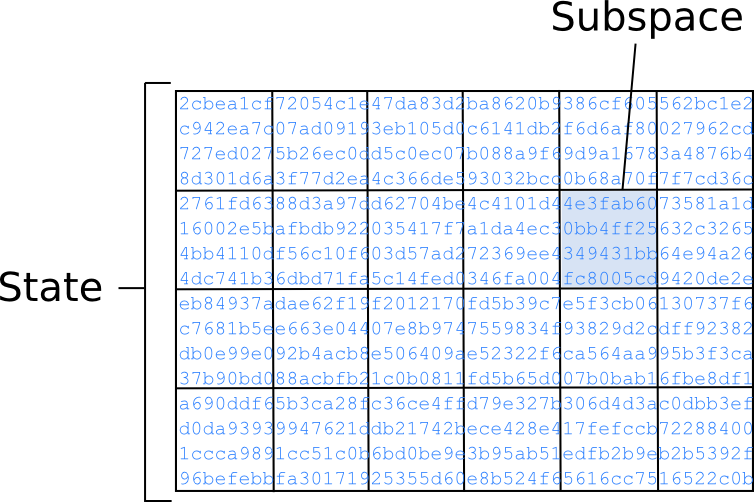
\includegraphics[width=190pt]{subspace2.png}
\end{center}

\begin{defn}[Affected area]
The \emph{affected area} of a transaction (or transaction list) $\tau$ in the context of $\sigma$ (denoted $\AFFECTED(\sigma, \tau)$) is the set of subspaces that were changed in the process of applying $\tau$, \ie the set of indices $S$ such that $(\sigma + \tau)[i] \ne \sigma[i]$ if and only if $i \in S$.
\end{defn}

\begin{center}
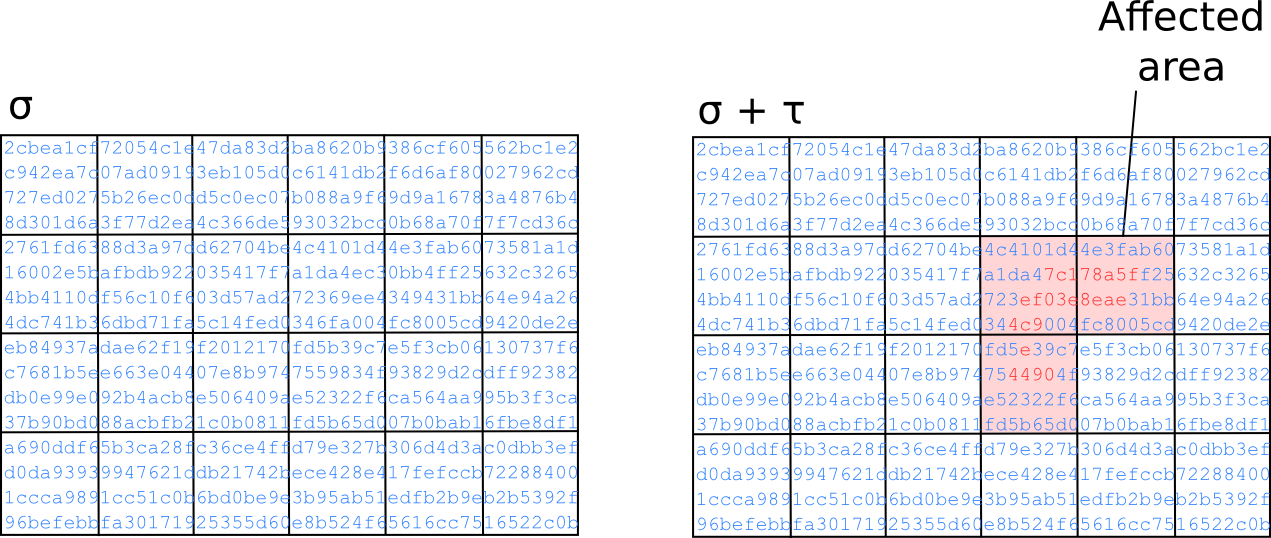
\includegraphics[width=300pt]{subspace1.png}
\end{center}

\begin{defn}[Observed area]
The \emph{observed area}, or in short \emph{area} (since observed area includes affected area), of a transaction (or transaction list) $\tau$ in the context of $\sigma$ (denoted $\AREA(\sigma, \tau)$) is the set of subspaces the values of which the result of the transaction depends on, \ie the smallest set of indices $S$ such that (i) $S \supset \AFFECTED(\sigma, \tau)$, and (ii) for any $\psi$ where $\psi[i] = \sigma[i]$ for $i \in S$ (but potentially $\psi[i] \ne \sigma[i]$ for one or more $i \notin S$), if we define $\psi' = \psi + \tau$ and $\sigma' = \sigma + \tau$, we have $\psi'[i] = \sigma'[i]$ for $i \in S$.
\end{defn}

\begin{note}
If we define a \emph{candidate observed area} as a set of indices as defined above, but not necessarily \emph{the smallest one}, we can show that the set of candidate observed areas is closed under intersection (basically, if $x$ is independent of anything outside $A$ and is independent of anything outside $B$, then it's independent of anything outside $A \cap B$), and so the concept of a ``smallest candidate observed area'' is unique and meaningful.

Ultimately, the observed area is incomputable; to see why, note that a state transition execution may contain an obfuscated circuit which grabs a value from a subspace and, unbeknownst to any conceivable generic analysis tool, multiplies it by zero (one can prove equivalence to the halting problem by constructing a program which runs the state transition function with all possible values for some subspace and halts only if it finds two values that lead to a different result). However, we can get a close approximation by simply adding a wrapper to the state transition execution code that keeps track of all subspaces that were accessed. We can use this as the ``observed area'' defined in the protocol.
\end{note}

\begin{center}
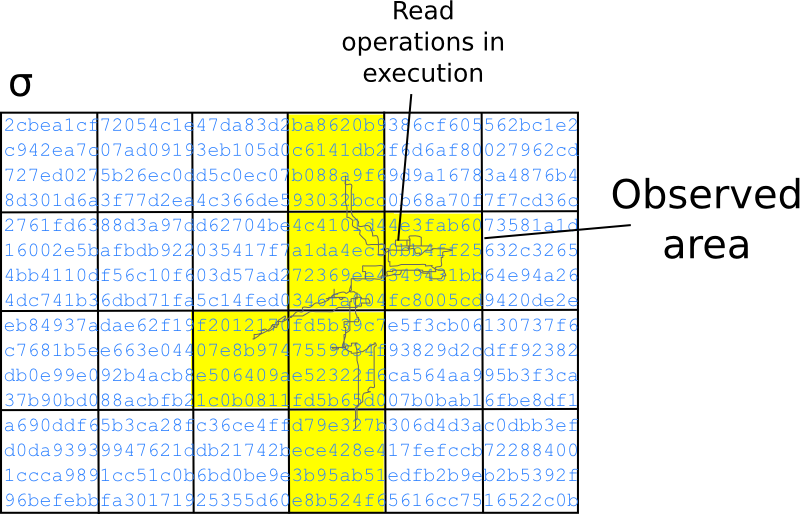
\includegraphics[width=190pt]{subspace3.png}
\end{center}

The concept of ``area'' is a key component our mechanism for collating transactions and parallelizing execution across the entire network; it allows transactions to be broken up into groups that can be processed at once by a few nodes that happen to fully possess that particular set of subspaces. If two transaction lists have completely disjoint areas, then we know that they can be computed in parallel. Technically, there is an even weaker condition that is sufficient for parallelizability: the \emph{affected area} of each transaction must be disjoint with the (total) \emph{area} of the other. Two observed areas intersecting with each other is not an issue. We will take advantage of this insofar as all transactions are aware of the header chain, but will otherwise employ the stronger criterion for establishing parallel evaluability for simplicity.

\begin{defn}[Sampling function]
A \emph{sampling function} is a function $\SAMPLE(W, k, m) \rightarrow {u_1 ... u_m}$ that takes a weight function $W$, a seed $k$ and a number $m$ and outputs a pseudorandomly selected (weighted by $W$) sample of $m$ users.
\end{defn}

\begin{exmp}
Arrange all users $u_1 ... u_n$ in order of public key, and assign the range $[\sum_{i=1}^{j-1} W(u_i)...\sum_{i=1}^j W(u_i)]$ to user $u_j$ for all $1 <= j <= n$. For all $1 \le h \le m$, return the user whose range includes the value $\frac{H(k + h)}{2^{256}}$ for some hash function $H$.
\end{exmp}

\begin{defn}[Merkle tree]
A Merkle tree\cite{merkle} is a mechanism for hashing a large piece of data, which in its most general form works as follows:
\begin{itemize}
\item
Use a partition function to split the data into chunks $D[1] ... D[n]$, such that each $D[i]$ has a very small size. Let us define this collection as $L_0(D)$.
\item
To determine $L_{i+1}(D)$ (starting from $i = 0$), split $L_i(D)$ into collections of fixed size (\eg 2-16 items) using some deterministic algorithm, and return as $L_{i+1}(D)$ the set of the hashes of the collections. Because there are fewer collections than elements (as each collection has more than one element), the size of $L_{i+1}(D)$ will be less than the size of $L(D)$
\item
Eventually, this leads to some $L_k(D)$ which has only one element. We call this the \emph{root} of the tree.
\end{itemize}
\end{defn}

In a standard Merkle tree, the ``collections'' are always made up of two adjacent elements, \eg if the original data has 32 elements, then $L_1(D)$ is made up of $H(D[1] + D[2])$, $H(D[3] + D[4])$, etc, then $L_2(D)$ is made of up $H(L_1(D)[0] + L_1(D)[1])$, $H(L_1(D)[2] + L_1(D)[3])$, etc. In a Merkle Patricia tree\cite{mpt} used in Ripple and Ethereum, the structure is somewhat more complicated, but with the benefit of greater flexibility in the case where elements are added or deleted from the partition. We are interested in Merkle trees because they can be used to implement two particular very powerful primitives:

\begin{defn}[Root function]
A \emph{root function} is a mapping $R(\sigma) = i \in D$ where $D$ is some domain, usually $\{0,1\}^{256}$, which is preimage-proof and collision resistant, and which also has the property that given a small change to $\sigma$ (\ie changes which have a small affected area according to some partition function), one can very quickly evaluate the new root, even if $\sigma$ is very large.
\end{defn}

\begin{defn}[Merkle proof protocol]
A \emph{Merkle proof protocol} is a scheme consisting of two functions:
\begin{itemize}
\item
$PROVE(\sigma, i) \rightarrow \pi$, taking as inputs a state $\sigma$ and an index $i$ and providing an output $\pi$, a ``proof'' showing that $\sigma[i]$ is indeed a part of $\sigma$
\item
$VERIFY(\rho, i, \pi, V) \rightarrow \{0, 1\}$, taking as input a state root $\rho$, an index $i$, a proof $\pi$ and a candidate value $V$. The function should only return 1 if $\pi$ is a proof showing that $V = \sigma[i]$ for some $\sigma$ such that $R(\sigma) = \rho$.
\end{itemize}
$PROVE$ and $VERIFY$ should both take logarithmic time.
\end{defn}

\begin{defn}[Merkle branch]
A \emph{Merkle branch} is the tuple $(V, \pi)$.
\end{defn}

\begin{note}
The above two mechanisms are interesting to us for two reasons. First, root functions prove a quickly updateable ``compact representation'' of a potentially very large piece of data; they are key in building our compact homomorphism for scalable blockchains. Second, Merkle proofs allow us to use this compact representation, in collaboration with the network supplying data, to securely determine any particular part of the underlying data that we may want to access.
\end{note}

\begin{defn}[Cryptoeconomically secure entropy source]
A cryptoeconomically secure entropy source is a protocol inside of a state transition function in a cryptoeconomic state machine that maintains an internal, regularly changing, value $v \in D$ for some domain $D$ (usually $\{0,1\}^{256}$) with the following desired properties:
\begin{itemize}
\item \emph{Unpredictablity}: there exists a value $M$ such that at time $t_0 + M$ the probability distribution of $v$ conditional only on information available at time $t_0$ is statistically indistinguishable from the random distribution. That is, an agent with only information available at time $t_0$ cannot determine a value $x$ such that $v = x$ with probability that is not in the range $[\frac{1 - \epsilon}{|D|}, \frac{1 + \epsilon}{|D|}]$ for cryptographically negligible $\epsilon$.
\item \emph{Upward uninfluenceability (I)}: For any predicate $P$ which the value $v$ would have at some given future time with probability $p$ assuming everyone correctly follows the specified protocol, the cost of making the value have that predicate with probability $p' > p$ is bounded below by $b * L * (p' - p)$ where $b$ is a constant independent of $P$ and $L$ is some economic metric of activity in the state machine.
\item \emph{Upward uninfluenceability (II)}: There exist constants $k$ and $b$ such that for any predicate $P$ which the value $v$ would have at some given future time with probability $p$ assuming everyone honestly follows the protocol, an actor controlling less than $k$ of the weight can increase the probability to at most $p' = p * (1 + b)$.
\end{itemize}
\end{defn}

\begin{exmp}
The cryptoeconomically secure entropy source used in NXT\cite{nxtinside} is defined recursively as follows:
\begin{itemize}
\item
$E(G) = 0$
\item 
$E(\sigma + \beta) = sha256(E(\sigma) + V(\beta))$ where $V(\beta)$ is the block proposer of $\beta$.
\end{itemize}
\end{exmp}

\begin{assm}
For any time internal $I$, there exists some fixed probability $p_o(I)$ such that a node randomly selected according to the weight function used to measure a cryptoeconomic state machine's Byzantine fault tolerance can be expected to be offline for at least the next $I$ seconds starting from any particular point in time with at least probability $p_o$.
\end{assm}

\begin{note}
Combining the two uninfluenceability criteria into one (``it is impossible to increase the probability of $P$ from $p$ to $p * (1 + k)$ without expending at least $b * L * k$ resources'') is likely very difficult; it is hard to avoid having ways to cheaply multiply the probability of low-probability predicates by only acting when you are sure that your action will have an influence on the result. 
\end{note}

\begin{note}
In practice, the second criterion is important for security, whereas the first criterion is important in order to avoid triggering superlinear returns on capital in systems where randomly selected stakeholders are rewarded.
\end{note}

\begin{lem}
The NXT algorithm described above satisfies the conditions for being a cryptoeconomically secure entropy source.
\end{lem}
\begin{proof}
To prove unpredictability, we note that the NXT blockchain produces a block every minute, and so the update $v \leftarrow sha256(v, V(\beta))$ takes place once a minute. During each round of updating, there is a probability $1 - p_o(60)$ that the primary signer will be online, and $p_o(60)$ that the signer will be offline and thus a secondary signer will need to produce the block. Hence, after $\frac{1}{-log(p_o(60))}$ blocks, there is a probability $p \approx \frac{1}{2}$ that the resulting value will be the ``default value'' obtained from updating $v$ with the primary signers' public keys at each block, and a $p \approx \frac{1}{2}$ probability that the resulting value will be different. We model 512 iterations of this process as a tree, with all leaves being probability distributions over sequences of 512 public keys of signers, where all probability distributions are disjoint (\ie no sequence appears with probability greater than zero in multiple leaves). By random-oracle assumption of $sha256$, we thus know that we have a set of $2^{512}$ independently randomly sampled probability distributions from $\{0,1\}^{256}$, and so each value will be selected an expected $\{0,1\}^{256}$ times, with standard deviation $2^{128}$. Hence, the probability distribution is statistically indistinguishable from a random distribution.
 
To show that the first uninfluenceability criterion holds true, note that the only way to manipulate the result is for the block proposer to disappear, leading to another proposer taking over. However, this action is costly for the proposer as the proposer loses a block reward. The optimal strategy is to disappear with probability $0 < q <= 1$ only when the predicate will be unsatisfied with the proposer participating but will be satisfied with the next proposer partipating; if a predicate has probability $p$ this entails disappearing $p * (1-p) * q$ of the time, meaning that the predicate will be satisfied $p + p * (1-p) * q$ of the time instead of $p$ of the time, a probability increment of $p * (1-p) * q$ will have a cost of $p * (1-p) * q * R$ if $R$ is the signing reward (whose real value is proportional to the quantity of transaction fees, a reasonable metric of economic activity). Hence, the desired condition holds true with $b = 1$.

To show that the second uninfluenceability criterion holds true, note that when one is not the signer, one has no influence on the entropy, and when one is the signer one has the ability to not sign and instead defer to the next signer. Hence, an attacker controlling $\frac{1}{k}$ of all signing slots will be able to defer to the second signer $\frac{1}{k}$ of the time, to the third signer $\frac{1}{k^2}$ of the time (by being in the first two slots simultaneously), etc, so in total such an attacker will on average be able to choose between $1 + \frac{1}{k-1}$ values and thus multiply the probability of a desired predicate by a factor of $1 + \frac{1}{k-1}$. If the attacker controls $\frac{1}{3}$ of all signing slots, the result will thus be increasing the probablity by a factor of $\frac{3}{2}$.
\end{proof}

\begin{note}
The above algorithm is only one of a class of algorithms that try to derive entropy from individual faults. There are also other approaches for deriving entropy, including $N-of-N$ commit-reveal protocols, relying on at least one of the participants to be altruistic and refuse to share their entropy with the other participants. It is an open problem to determine if one can come up with cryptoeconomically secure entropy sources cheaper than proof-of-work that rely purely on a rationality assumption.
\end{note}

\begin{note}
The above algorithm is NOT \emph{downward-uninfluenceable}. If there is a predicate $P$ with low probability, then one can influence its probability down to $P * w_a$ by simply bribing all validators who would have created a block that changed the entropy value to something satisfying $P$ to instead sit their turn out and let the next validator make a block, almost certainly not triggering $P$. The $w_a$ multiplier comes from the fact that we are assuming a subset of ``altruistic'' validators that cannot be bribed. However, for predicates with medium probability, one can derive a certain degree of resistance to downward influence simply by applying the upward-uninfluenceability guarantees to $\neg P$.
\end{note}

\begin{defn}[zk-SNARK scheme]
A zk-SNARK scheme is a tuple of three functions $G$, $P$, $V$, where:
\begin{itemize}
\item
$G(prog) \rightarrow k$ generates a ``verification key'' from a program.
\item
$P(prog, I_s, I_p) \rightarrow \pi$ generates a proof that $prog(I_s, I_p)$ for some secret inputs $I_s$ and public inputs $I_p$ is equal to its actual output, $o$.
\item
$V(k, I_p, o, \pi) \rightarrow \{0, 1\}$ verifies a proof, accepting it only if $\pi$ is actually a proof that $prog(I_s, I_p) = o$ where $G(prog) = k$.
\end{itemize}
Essentially, it is a proof that you ran a particular computation with some particular inputs and got a particular result, such that the proof can be verified much more quickly than running the original computation. Additionally, to qualify as a \emph{zero-knowledge} ZNARK, $\pi$ should reveal no information about the value of $I_s$. Schemes exist \cite{snark} to perform $G$ and $P$ in a time equal to $O(N*log^k(N))$ for a small $k$ where $N$ is the number of execution steps, and $V$ can be computed in some cases in polylogarithmic time and in some cases in constant time.
\end{defn}

\begin{note}
We provide algorithms which achieve scalability without zk-SNARKs, however we will show how zk-SNARKs can also be used in scalable blockchain protocols.
\end{note}

\begin{defn}[Decentralized oracle scheme]
A decentralized oracle scheme is a mechanism which asks a set of participants to provide an answer to a subjective question (\eg ``what was the temperature in San Francisco on 2015 Jan 9?''), and attempts to incentivize the participants to answer correctly. The output of the mechanism is generally considered to be the majority answer, and as input the scheme usually requires an economic subsidy.
\end{defn}

\begin{exmp}
A simple decentralized oracle scheme, called ``SchellingCoin'', has the following rules:
\begin{itemize}
\item
Each of $N$ participants must vote either $1$ or $0$ on a question (a scalar-valued or multi-valued question is modeled as a series of binary questions).
\item
A participant whose vote aligns with the majority vote receives a reward of $P$.
\item
A participant whose vote does not align with the majority vote receives a reward of $0$.
\end{itemize}
SchellingCoin is vulnerable to zero-cost equilibrium flips, and so under a formal definition of economic security it cannot be viewed as having any security margin at all, though the difficulty of the inherent coordination problem may still allow the scheme to function in practice. An attacker with a budget greater than $P$ and the ability to credibly commit to to providing a bribe under certain conditions in the future can, assuming rationality of the participants, effect an equilibrium flip toward a wrong answer at no cost \cite{pepsilon}.
\end{exmp}

\begin{note}
There are two ways to make SchellingCoin-like protocols more powerful by increasing their security margin. The first involves a strategy of Sztorcian counter-coordination\cite{sztorc}, which attempts to naturally set the quantity of funds at stake in proportion to the level of controversy in the question; in the limit, people who do not vote alongside the majority answer lose their entire security deposit. The game-theoretic argument that Sztorc provides\cite{sztorc2} is that if a medium-sized bribe to vote incorrectly is offered, then voters will vote for the correct answer with some of their funds and for the incorrect answer with some of their funds, leading to an equilibrium where the majority of the voting power is still in favor of the correct answer but the users also manage to ``steal'' some of the bribe:

\begin{center}
\includegraphics[width=165pt]{schellingcoin_payoff1.png}
\includegraphics[width=165pt]{schellingcoin_payoff2.png}
\end{center}

This approach accepts that attackers with a budget even larger than the size of everyone's security deposits will be able to cause everyone to flip to voting incorrectly as an equilibrium, but advocates note that attackers that large will also be able to arbitrarily disrupt the underlying blockchain consensus anyway.

The second is to fall back to ``subjective resolution'': if the majority of voters vote incorrectly, then it is up to \emph{the users} to simply reject that block as invalid and go along with the block that they see as correct. This reliance on human judgement at the last level makes the budget required for any kind of zero-cost ``equilibrium flip'' attack essentially infinite, instead requiring the attacker to bribe everyone outright and even then resulting in only a moderately large inconvenience for users, not a total failure. The process does impose inconveniences to users, but properly built designs that use decentralized oracle schemes will use the mechanism only as the last step of a fallback game in a similar function as nuclear deterrence; in practice it will almost never be used. The security claim essentially becomes something like ``by paying \$100 million, an attacker has the ability to force users to visit their favorite internet forum and locate a 32-byte hash representing the new fork of the chain to switch to''.
\end{note}

\begin{defn}[Distributed hash table]
A distributed hash table is a mechanism which stores a potentially very large number of chunks of data on a decentralized network in order to allow network-connected nodes easy access to them. For our purposes, we are particularly interested in a \emph{verifiable decentralized data store} which gives network-connected nodes access to a function $\GET(\rho, i) \rightarrow (V, \pi)$ where $(V, \pi)$ is the Merkle branch of $\sigma[i]$ where $\rho = R(\sigma)$; however, given that Merkle tree protocols consist simply of repeated reverse-hash-lookup queries, this definition can easily be deduced from the more conventional definition of providing a function $\GET(h) \rightarrow x$ where $h = H(x)$ for some hash function.
\end{defn}

\begin{note}
$\GET$ should work with overwhelmingly high probability provided that (i) $(V, \pi)$ has at least once been in the hands of at least one altruist, and (ii) the total quantity of data stored in the DHT is at most $\frac{N * n}{k}$ where $N$ is the computational and data storage capacity of a node, $n$ is the number of nodes and $k$ is a constant. We will generally assume that there is an upper bound on the average number of nodes interested in a particular subspace, and so in the rest of this document we will simply assume that the DHT works.
\end{note}

\begin{exmp}
Kademlia \cite{kademlia} is an example of a distributed hash table. A more direct implementation of our desired formalism with Merkle branches will be available from IPFS \cite{ipfs}.
\end{exmp}

\section{Global Variables and Assumptions}

In the rest of this document we will use the following variables:

\begin{itemize}
\item
$N$ - the maximum computational power of a node
\item
$L$ - the level of economic activity in the network
\item
$m$ - the size of the randomly selected pool of validators that need to validate each block (usually 50 or 135)
\item
$n_s$ - the number of subspaces
\item
$n_t$ - the number of transactions per collation
\item
$n_c$ - the number of collations per block
\item
$D$ - the size of a validator security deposit
\item
$r$ - the reward for a validator to sign a particular collation
\end{itemize}

$\tau$ will represent transactions, $\beta$ will represent blocks and block headers depending on context, and $B$ will represent ``super-blocks''. We also make the following assumptions:

\begin{itemize}
\item
There exists some constant $w_a$ such that at least $w_a$ of weight is altruistic (\ie willing to follow the protocol even ignoring the potential for greater monetary gains from violating it)
\item
The number of transactions, the potential budget of attackers, the potential budget of altruists, and any economic metric of activity $L$ that we use for the purposes of measuring economic security are all proportional to each other.
\item
Moderate wealth concentration: there exist many individuals that hold at least $\frac{L}{N}$ wealth.
\item
There exists some fixed number $k_t$ such that most transactions observe and affect at most $k_t$ subspaces.
\item
There exists some fixed number $k_u$ such that on average a user is interested in accessing data from at most $k_u$ subspaces.
\item
As soon as data makes it into the hands of at least one altruist, it will propagate through the distributed hash table and become available to everyone.
\item
The underlying top-level consensus algorithm works, and has all security properties that are desired.
\item
The underlying top-level consensus prevents censorship of transactions in the long term; \ie there is some period of time $T_c$ within which a transaction will almost certainly be accepted into the network.
\end{itemize}

\section{A Byzantine-fault-tolerant Scalable Consensus Overlay}

Now, let us define the core part of our scheme. As described in a previous section, the mechanism can most simply be formally described as using any underlying consensus algorithm to keep track not of the state, but of a compact homomorphism (``top level'') of the state, and then building separate (``bottom-level'') machinery to collaboratively ensure that the underlying state transitions are legitimate.

The basic mechanism is this. Suppose that $\sigma$ is partitioned using some partition function into $n$ parts. If $\sigma$ is partitioned into a map $\{i: \sigma[i]\}$, we define $\psi$ as the map $\{i: R(\sigma[i])\}$. We assume the existence of a coarse-grained partition function as well as the existence of a fine-grained partition function which converts $\sigma[i]$ into a map $\{j: \sigma[i][j]\}$, where each $\sigma[i][j]$ is constant-size (\eg an account). We then define an object called a \emph{transaction collation}, which consists of three components:

\begin{itemize}
\item
$T$, a list of transactions
\item
A \emph{header} $H$, consisting of:
    \begin{itemize}
    \item
    $AP$, the set of previous state roots $\{i: R(\sigma[i])$ for $i \in \AREA(\sigma, T)\}$
    \item
    $AN$, the set of new state roots $\{i: R(\sigma'[i])$ for $i \in \AREA(\sigma, T)\}$
    \item
    $S = [s_1 ... s_m]$, an array of signatures
    \item
    $R(T)$ (the root hash of the list of transactions)
    \end{itemize}
\item
$D$, the set of Merkle branches for the observed area of $T$ on $\sigma$ on the fine-grained partition level.
\end{itemize}

We also add to the top-level state $\psi$ a pool of validators $V(\psi)$. In order to achieve economic security, we will later recommend that these validators hold security deposits, but if super-protocol social mechanisms are allowed to play a dominant regulatory role then some security can be achieved under the weaker condition that the validators have persistent identities, and if the only goal is Byzantine fault tolerance and not economic security then all that matters is that it is hard to become a validator and there are many of them. Ideally, top-level consensus participants (\eg Tendermint stakeholders, miners) and validators would be the same group.

Additionally, we add a cryptoeconomically secure entropy source, $E(\psi)$. Finally, we select some sample function, and we define $\VALIDATORS(H, \psi) = \SAMPLE(W, E(\psi) + AP, m)$, selecting $m$ random validators for the collation using the entropy source $E$ and the previous state root set $AP$, as a source of entropy (we need additional entropy alongside $E$ so as to ensure that different collations have different validator pools, and $AP$ is used (in sorted order) because modifying it is expensive: removing a state root requires throwing away transactions, and adding a state root requires taking up space, making the entity including the transaction have to pay the opportunity cost of including another collation in that spot). An alternative is to simply use a small amount of proof of work as the secondary source of randomness; this will also help decrease the number of collations to a manageable quantity.

When a collation is passed around the network, the entire ensemble $\kappa = (T, H, D)$ is included. From the point of view of the top-level consensus, however, only $H$ exists, and $H$ ends up playing the role of a ``transaction'' from the top-level consensus's point of view. For the purposes of defining $\APPLY'$, the top-level state transition function, we say that a collation header $H$ is valid in the context of $\psi$ if and only if the following are all true:

\begin{itemize}
\item
For all $i \in AP$, $\psi[i] = AP[i]$ (\ie the collation's pre-state matches up with the actual pre-state)
\item
$S$ includes valid signatures from at least two thirds of $\VALIDATORS(H, \psi)$
\end{itemize}

If $H$ is valid, we set $\psi'$ by:

\begin{itemize}
\item
For all $i \in \AREA(\sigma, T)$, $\psi'[i] = AN[i]$
\item
For all $i \notin \AREA(\sigma, T)$, $\psi'[i] = \psi[i]$
\end{itemize}

The top-level state transition function has an additional validity constraint: for the block to be valid, the areas of all collation headers included must be disjoint from each other. The underlying consensus algorithm will keep track of blocks, where each block contains a number of collation headers, and we will refer to the blockchain produced by the underlying consensus algorithm as the \emph{header chain}.

Now, let us specify the bottom-level validation criteria. These are not placed into the top-level state transition function (although in later sections we will modify the protocol to require top-level consensus participants to all perform specific bottom-level validations \emph{in extremis} in the event of serious attacks); rather, they can be viewed as ``suggestions'' for when validators should sign collations. The conditions are fairly simple and intuitive:

\begin{itemize}
\item
Every transaction in $T$ is valid in its context when applied to $\sigma$, the full pre-state associated with the compact pre-state $\psi$ of the header chain before the transaction.
\item
$D$, $AP$, and $AN$ are produced correctly.
\end{itemize}

In short, the validators validate that the transactions are actually valid. In practice, the way that they will do this is through one of two strategies. First, they may receive the collation directly from the entity that produced the collation, and the Merkle branch set $D$ gives them the specific information that they need from the observed and affected subspaces to re-compute the state transition function and ensure that the final subspace roots are correct. Second, they may receive the collation header, and download information from the distributed hash table on the fly.

Now, we will prove that our homomorphism is actually a homomorphism - \ie that $H$ is valid in the context of $\psi$ only if $T$ is valid in the context of $\sigma$, and that the final state $\psi + H$ is equal to $\{i: R((\sigma + T)[i])\}$ (\ie a correct compact representation of the final state) with extremely high probability as long as a Byzantine fault tolerance guarantee is satisfied: less than one third of the weight of validators is Byzantine. 

\begin{lem}
Assuming less than $\frac{1}{3}$ of the weight of validators is Byzantine, a block that is valid under the above top-level state transition function will produce a top-level state $\psi'$ such that if we define $\sigma'$ with $\sigma' = \{i: R^{-1}(\psi'[i])\}$, $\sigma' = \sigma + T_1 + T_2 + ...$ where $T_i$ is the set of transactions in $H_i$ where $H_i$ is the collation header root corresponding to the collation containing transaction list $T_i$.
\end{lem}

\begin{proof}
Suppose that all $\beta_i$ satisfy the second-level validity criteria. Then, note that each subspace in $\sigma$ is only modified by at most one $T_i$, and so we can model the state as a tuple $(O, A_1, A_2, A_3 ... A_n)$ if $\beta$ includes $k$ transactions, where $A_i$ is the affected area of $T_i$ and $O$ is the remaining part of $\sigma$. The state after $T_1$ will be $(O, A'_1, A_2, A_3 ... A_n)$, by disjointness the state after $T_2$ will be $(O, A'_1, A'_2, A_3 ... A_n)$, and so forth until the final state is $(O, A'_1, A'_2, A'_3 ... A'_n)$. If we use the top-level state transition function on $\psi$, we can partition $\psi$ similarly into $(O, B_1, B_2, B_3 ... B_n)$, and a similar progression will take place, with state roots matching up at every step. Hence the final state at this top-level state transition will be made up of the roots of the subspaces in $\sigma'$.

Now, suppose that one $\beta_i$ does not satisfy the second-level criteria. Then, validators following the protocol will consider it invalid, and so $\frac{2m}{3}$ validators will not be willing to sign off on it with very high probability, and so the block will not satisfy the top-level criteria.
\end{proof}

Hence, we know that the resulting $\psi'$ will represent a state which is \emph{valid}, in the sense that it can be described as a series of transactions applied to the genesis. This is the validity criterion that we will repeatedly use in order to prove that validity is preserved by other mechanisms that we introduce such as revert mechanics.

Because a sampling scheme is inherently probabilistic, it is theoretically prone to failure, and so we will precisely calculate the probability that the protocol will fail. Assuming a 96-bit security margin, we can consider a probability negligible if the average time between failures is longer than the time it takes for an attacker to make $2^{96}$ computations. If we assume that the cryptoeconomically secure entropy source updates every super-block, and a super-block comes every 20 seconds, then one can reasonably expect a hostile computing cluster to be able to perform $2^{48}$ work within that time, so we will target a failure probability of $2^{-48}$ (this implies roughly one failure per 445979 years of being under attack). We can determine the failure probability with the binomial distribution formula:
\\
\\
$\PE(n, k, p) = p^k * (1-p)^{n-k} * \frac{n!}{k!(n-k)!}$
\\
\\
Where $\PE(n, k, p)$ is the probability of an event that occurs with probability $p$ in an attempt will achieve exactly $k$ occurrences out of $n$ attempts. For convenience, we define $\PGE(n, k, p) = \sum_{i=k}^n \PE(n, i, p)$, \ie the probability of \emph{at least} k occurrences.

We note that $\PGE(135, 90, \frac{1}{3}) = 2^{-48.37}$, so 135 nodes will suffice for a $k = \frac{1}{3}$ fault tolerance. If we are willing to lower to $k = \frac{1}{5}$, then $\PGE(39, 31, \frac{1}{5}) = 2^{-48.58}$, so 39 nodes will be sufficient. Additionally, note that if we want greater efficiency under normal circumstances, then a bimodal scheme where either 44 out of a particular 50 nodes ($\PGE(50, 44, \frac{1}{3}) = 2^{-49.22}$) or 90 out of a particular 135 nodes is a sufficient validity condition will allow the cheaper but equally safe condition to work in the (usual) case where there are almost no malicious nodes, nearly everyone is online and the network is not under attack, and fall back to the more robust but bulkier validation rule under tougher conditions.

Additionally, note that the combinatoric formula is only valid if the entropy used to determine validator sets is \emph{actually} random, or at least close enough for our purposes. For this, our second uninfluenceability criterion, stipulating that an attacker with less than $\frac{1}{3}$ of all validators will be able to influence it by at most a reasonably small linear amount (in the NXT case, by a factor of $\frac{3}{2}$), is crucial, showing that with such a powerful attacker the probability of a successful attack remains below $2^{-47.4}$. The first uninfluenceability criterion is important in order to avoid excessive superlinear returns resulting from super-block proposers manipulating the entropy in order to increase the chance that their validators will be involved in verifying blocks, but does not affect security.

To see the role of the unpredictability criterion, note that the protocol as described here provides \emph{ex ante} Byzantine fault-tolerance, but not \emph{ex post} Byzantine fault tolerance; \emph{after} the validators are selected, only that small fixed number of validators acting maliciously will compromise the system. If entropy becomes unpredictable very slowly (or never at all), then the algorithm is only Byzantine fault-tolerant against faults very far in advance, leading to potential practical vulnerabilities like an attacker locating the 135 validators that will be validating their block one year from now and taking the time to locate and hack into 90 of them.

\begin{lem}
The above protocol is almost-quadratically scalable, in the sense that it does not require any individual to perform more than $O(N)$ work even if the total transaction load is $O(N^{2-\epsilon})$.
\end{lem}

\begin{proof}
Suppose that the size of a collation is calibrated correctly: each block contains $n_c \in O(N^{1-\epsilon})$ collations, each collation contains $n_t \in O(N^{1-\epsilon})$ transactions, the number of subspaces is also at $n_s \in O(N^{1-\epsilon})$, and that there are $n_v \in O(N^{1-\epsilon})$ bottom-level validators. We leave it to the protocol to determine how to auto-calibrate these values; we provide some suggestions in a later section.

First, let us consider the workload of a top-level consensus participant. A top-level consensus participant must validate $n_c$ collations, where each collation contains $m$ signatures, as well as data associated with some number of subspaces. The total number of subspaces in all collations is at most $n_s$, since each subspace can be used by at most one collation. If it takes $e_{sig}$ computational effort to download and verify a signature, and $e_{col}$ computational effort to download and verify a subspace root, then the total effort of processing a block will be at most $e_{col} * n_s + e_{sig} * m * n_c \in O(N^{1-\epsilon})$. Supposing that a validator registration takes $s_v$ space, and a subspace takes up $s_s$ space (realistically, $s_s = 32$ bytes and $s_v < 100$ bytes), the size of the state is equal to $n_v * s_v + n_s * s_s \in O(N^{1-\epsilon})$. We can assume logarithmic overhead from the Merkle tree verifications, but even still the total computational complexity and the size of all objects together remain below $O(N)$.

Now, let us consider the workload of each bottom-level validator. There are $n_v$ bottom-level validators, $n_c$ collations, and each collation must be approved by $m$ validators; hence, if one collation takes $E$ effort to validate by one validator, the total work is $E * n_c * m$, and the total work per validator is $\frac{E * n_c * m}{n_v}$ (because the validators are chosen randomly, we assume that the workload is evenly distributed, and validation is not compulsory so even if exploitation opportunities exist that is not a valid denial-of-service vector). Because there are $n_t \in O(N^{1-\epsilon})$ transactions, we can conclude $E \in O(N^{1-\epsilon})$, and so $\frac{E * n_c * m}{n_v} \in O(N^{1-\epsilon})$. The transactions and Merkle proofs would take up $O(N^{1-\epsilon} * log(N)) < O(N)$ space, so the storage and bandwidth load is also manageable.
\end{proof}

The incentives inside such a scheme would be provided as follows:

\begin{itemize}
\item
Transactions can pay transaction fees to the producer of the block that includes them.
\item
Blocks can pay transaction fees to the proposer of the super-block that includes them, as well as the the validators that will sign off on them.
\item
The proposer of the super-block can pay transaction fees to the validator pool of the super-block; this fee can be mandatory (\ie protocol-enforced) or enforced by validators refusing to sign a block with a fee that is too small for them.
\item
The protocol may optionally add a mandatory fee to transactions and blocks, and this fee can get destroyed. The protocol may also add an \emph{ex nihilo} reward to the validators of the super-block in place of requiring it to be paid from transaction fees.
\end{itemize}

\section{Economic Security}

The previous algorithm provided a statistical guarantee of data availability and validity by simply assuming that at least two thirds of validators are honest; however, it carries an inherent fragility: if, for any reason, a small sample of nodes actually does end up signing off on an invalid block, then the system will need to hard-fork once the fault is discovered. This results in three practical weaknesses:

\begin{itemize}
\item
Larger safety factors are required on the sample sizes in order to ensure that a sample is absolutely never malicious. If there was a way of recovering from a bad collation entering the system, the number of validators required to sign every collation could be substantially decreased, increasing normal-case efficiency.
\item
The economic security of the algorithm scales only with $N$ and not with $L$: in order for an attacker to produce an invalid collation that gets accepted by the above algorithm, they need only bribe $\frac{2m}{3}$ out of a pool of $m$ validators, with a total cost of $D * \frac{2m}{3} \in O(N) < O(L)$. Sampling provides security against random faults, but bribery allows attackers to create targeted faults after the fact.
\item
Even in the absence of bribing attackers, there is an incentive for validators to simply be lazy and sign every collation - particularly once they see that every collation that has appeared so far is legitimate.
\end{itemize}

If we are content with the large safety factors, one approach to dealing with the issue is to not bother with economic security, and instead simply rely on Byzantine-fault-tolerance guarantees. In order to ensure that the majority of validators are beneficent, we ask top-level consensus participants to censor attempts to join the validator pool by parties that appear to be unreliable or likely to be malfeasant - essentially, a protocol-wide know-your-validator regime. In some cases, particularly regulated financial systems, such restrictions are necessary in any case and so we need to go no further\cite{swanson}. If we are trying to create a more open network, however, then such a solution is unsatisfactory, and so we arguably need not just Byzantine fault tolerance but also regulation via economic incentives.

We will generally operate within the following framework:

\begin{itemize}
\item
There exists a ``challenge'' mechanism by which anyone can pay a cost $c_c$ in order to challenge what they perceive to be an invalid collation. Note that we need $c_c \in O(N^{1-\epsilon})$; if challenges are cheaper, then an attacker will be able to overwhelm the header chain by producing more than $O(N)$ challenges at a cost of $O(L) = O(N^{2-\epsilon})$.
\item
If a collation is unchallenged for $F_d$ blocks, then it is considered ``finalized''.
\item
If a collation is challenged, then it is placed in ``purgatory''. If it remains in purgatory for $P_d$ blocks, then the collation is reverted (we will determine the precise mechanics of reversion in a later section), and the challenger receives the security deposits of the original $m$ validators of the collation as well as any redeemers (see below).
\item
If a collation is challenged, then a larger randomly selected set of $2 * m$ validators must attest to the validity of the collation in order to ``redeem'' it. Challengers can optionally pay a higher cost $k * c_c$ in order to make the required redemption set even larger, $2 * k * m$, right up to a maximum of the entire set of $n_v$ validators.
\item
Participating in a redemption has some very small economic reward (note that only a small reward is required, because a validator can know for sure that they are redeeming a valid and available collation, and that they will be able to convince others of this, by simply downloading it themselves).
\item
If a collation is redeemed, then the $F_d$ period begins again, and the collation can be challenged again within that period - although this time a minimum $k$ multiplier is placed at twice the multiplier of the last challenge. If challenges continue appearing, this will eventually escalate to all $n_v$ validators checking the collation. If a collation is finalized after being redeemed, the collation producer and validators are penalized slightly; this makes it costly to engage in ``crying wolf attacks'' as described below.
\item
When all $n_v$ validators are checking the collation, we incentivize honesty by either using a decentralized oracle scheme, or by asking the \emph{top-level consensus process} to adjudicate: if a block contains a pool of $n_v$ validators attesting to a collation that is invalid, then we add a top-level rule saying that that block should be considered invalid.
\end{itemize}

The chief difficulty in providing economic security is that there are in fact two ways in which a collation can be invalid. The first is that a collation is produced and broadcasted normally, but the block either includes an invalid transaction or has an invalid final state root. In this case, the problem is easy; in fact, we can prove that under the above mechanism acting honestly is a subgame-perfect equilibrium. The second, and more difficult, kind of validity centers around data unavailability. An attacker may simply create a (valid or invalid) collation, publish the header, but refuse to publish the contents, making it impossible for the network to learn the complete final state.

The problem here is this: whereas in the case of invalid collations, the validity or invalidity of a collation is fixed and cannot change, in the case of unavailable data that is not the case. An attacker can always create an unavailable collation, wait for challengers to challenge, and then publish the data and start the redemption process, costing the challengers money. The attacker may do this again and again, draining challengers' resources, until eventually challengers no longer find it economically rational to challenge bad collations, giving the attacker free rein to push through invalid collations; we call this the \emph{crying wolf attack}.

Although it may seem like data availability is less serious a problem than invalidity, we will provide a series of attacks to show that the ability to push through in some cases even valid unavailable collations can be a death knell to a working blockchain system:

\begin{exmp}[Unprovable theft attack]
An attacker creates a block with transactions $T_1$ ... $T_n$, where $T_1$ ... $T_{n-1}$ are legitimate and applied properly but $T_n$ is an invalid transaction which seems to transfer \$1 million from an arbitrary wealthy user to the attacker. The attacker makes $T_1$ ... $T_{n-1}$ available, and makes the final state available, but does not make $T_n$ available. Once the state is confirmed by a sufficient number of future blocks, the attacker than spends the \$1 million to purchase other untraceable digital assets.

Here, note that there is no way to prove invalidity, because theoretically $T_n$ very easily \emph{could be} a transaction legitimately transferring \$1 million from the millionaire to the attacker, but the unavailability of the data prevents the network from making the judgement.
\end{exmp}

\begin{exmp}[Sudden millionaire attack]
An attacker creates a block with transactions $T_1$ ... $T_n$, where $T_1$ ... $T_{n-1}$ are applied properly but $T_n$ is an invalid transaction. The attacker then makes $T_1$ ... $T_{n-1}$ available, and makes \emph{most} of the final state available, with the exception of one branch where the attacker has given themselves \$1 million out of nowhere. Two years later, the attacker reveals this branch, and the network is forced to either accept the transaction or revert two years of history.
\end{exmp}

\begin{note}
One way to try to solve both attacks above is to require every valid transaction to show a valid ``source'' of its income. However, this leads to a recursive buck-passing problem: what if the attacker performs a sudden millionaire attack to create a new unexplained account $A_1$, then creates a block with an unavailable transaction sending funds from $A_1$ to $A_2$ (possibly a set of multiple accounts), then $A_3$, and so forth until finally collecting the funds at $A_n$, and then finally reveals all transactions upon receiving $A_n$. The total dependency tree of a transaction may well have total size $\omega(N)$. Peter Todd's tree-chains discussion offers the solution\cite{treechains} of limiting the protocol to handling a fixed number (possibly more than $O(N)$) of ``coins'', each one with a linear history; however, this solution is not sufficiently generalizeable and abstract for our purposes and carries high constant-factor overhead.
\end{note}

\begin{exmp}[Transaction denial attack]
An attacker creates a block with an unavailable transaction which appears to modify another party's account (or spend their UTXO). This prevents the other party from ever performing any actions with their account or their funds, because they can no longer prove validity.
\end{exmp}

\begin{note}
Even zk-SNARK protocols cannot easily get around the above problem, as it is information-theoretically impossible for any protocol regardless of cryptographic assumptions to fully specify the set of accounts that are modified in a particular super-block in $O(N)$ space if the set itself is greater than $O(N)$ in size.
\end{note}

\begin{exmp}[Double-spending gotcha attack]
Suppose that a protocol tries to circumvent payment-denial attacks by making payment verification a challenge-response process: a transaction is valid unless someone can show that it is a double-spend. Now, an attacker can create a block containing a legitimate but unavailable transaction that spends \$1 million from account $A_1$ to $A_2$, also controlled by them. One year later, the attacker sends \$1 million from $A_1$ (which no one can prove no longer has the money because the data is unavailable) to $A_3$. One year after that, the attacker reveals the original transaction. Should the network revert a year of history, or allow the attacker to keep their \$2 million?
\end{exmp}

\begin{note}
Zk-SNARK protocols are not a solution here either, because of the same information-theoretic issues.
\end{note}

In order to remove the possibility of such issues in the general case, we will try to target a hard guarantee: given a general assumption that once data is available at all it is guaranteed to remain available forever due to a combination of the DHT and altruist-operated archival services, we will attempt to ensure that, for all collations $\kappa$, it is the case that either all of $\kappa$ is available or $H$ is reverted by the top-level consensus (we will define the precise semantics of ``reverting'' in a later section).

If $N < \frac{D * m}{c_c}$ (where $D$ is the size of a validator deposit, with $D \in O(N^{1-\epsilon})$, and $c_c$ is the cost of challenging), then the crying wolf attack is not a problem. If a challenger discovers an invalid collation, and the collation is proven to be invalid, then the challenger receives a reward of $D * m$ from the security deposits of the validators that accepted the collation; hence, challenging makes economic sense if the perceived probability that an currently unavailable collation will remain unavailable is at least $\frac{c_c}{D * m}$. By the law of Laplacian succession\cite{laplace}, convincing rational challengers that the probability is less than this will require roughly $\frac{D * m}{c_c}$ unavailable collations that later become available, and if $\frac{D * m}{c_c} > N$, then the cost of doing so is greater than the cost of simply 51\% attacking the network head-on.

If $N > \frac{D * m}{c_c}$, however, then the situation is different, and the crying wolf attack actually does become the most cost-efficient way of compromising the system. In this case, we need to either concede that, \emph{in extremis}, challenging is an altruistic activity, or find some alternative mechanism of incentivizing challengers.

We can model the situation as a kind of law-and-economics problem: the ``crime'' is creating invalid collations, the ``police officers'' are challengers, and our job is to incentivize enough law enforcement activity to ensure that no crimes gets through uncaught. We will show two strategies for doing this, one roughly corresponding to ``private enforcement'', where individuals are motivated to participate by ``privatizing the loss'' of a successful collation getting through among a specific set of individuals, and the other roughly corresponding to ``public enforcement'', where a central common pool of funds is used to pay challengers, making the payments via a kind of lottery to minimize the amount of work required to make sure that challengers are doing their jobs.

We also make the assumption that, when a challenge is made against a genuinely unavailable collation, and the challenge is at such a level that the entire set of validators is required to participate in redeeming it, there is some fixed probability $p$ such that the validators will check for the collation's availability and conclude that it is unavailable even before the attacker can publish it. We can assume a small $p$, \eg $p \approx 0.001$; decreasing our estimate of $p$ simply makes the network linearly more vulnerable to denial-of-service attacks.

The private enforcement strategy works as follows. First, we withhold the reward for making a block (\emph{proposing} in Tendermint, \emph{mining} in Bitcoin, etc) for $F_d$ blocks, and keep it as a temporary deposit. Suppose that a collation is unavailable, and does not get challenged for $\frac{F_d}{2}$ blocks. Then, a challenger has the ability to place a challenge at cost $c_c * \frac{n_v}{m * 2}$ in order to require redemption by all validators. If the challenge succeeds, then the challenger receives the rewards (plus, for good measure, a portion of the deposits) of all block makers between the time of the block's creation and the block that includes the challenge.

This has two consequences. First, it increases the reward for a challenger to $\frac{F_d}{2} * R \in O(L)$ (where $R$ is the block reward), meaning that as long as $\frac{c_c * \frac{n_v}{m * 2}}{\frac{F_d}{2} * R} < p$, challenging is rational. The above equation can be re-written as $\frac{c_c * n_v * 2}{F_d * m * R}$, with the constants $F_d$ (we recommend $F_d \approx 40$) and $m$ (as in the previous section, we recommend $39 \le m \le 135$ depending on parameters) at the bottom, so the truth of the inequality is quite plausible, particularly with sufficiently small values of $c_c$. Second, it transforms deterrence against bad collations from a public good into a private good - if a bad collation makes it through the first $\frac{F_d}{2}$ blocks, then the next block makers specifically are liable. This creates the incentive for those block makers to subsidize challengers to challenge during previous blocks - perhaps privately using techniques like the random auditing that we will discuss for the public enforcement strategy later.

The public enforcement strategy works simply: every block, we use a small amount of proof of work, perhaps with expected per-block cost $w = R * 0.01$, as a source of entropy from which to select a random subspace. We then ask all top-level consensus participants to validate the last collation on that subspace. If that collation is indeed unavailable, and the block has been challenged, then the challengers split a reward of size $r_c = w * 0.49 \in O(N^{2-\epsilon})$. The block maker also gets a reward of equal size.

The scheme can be thought of an inverted application of a standard result from law and economics: one can achieve compliance with arbitrarily low enforcement cost by simply decreasing the level of enforcement, and thus the probability of getting caught, but simultaneously increasing the fine\cite{econofcrime} - except, in our case, we are performing the exact opposite task of a police department as we are trying to \emph{incentivize a virtuous usually-costly action} with the occasional application of a \emph{reward}. The load each validator is at most the cost of downloading one block, $O(N^{1-\epsilon})$, and each subspace will have a propbbility of at least $\frac{1}{O(N^{1-\epsilon})}$ of being randomly inspected; hence the scheme does not compromise scalability. However, assuming that a top-level challenge has at least a fixed probability $p$ of correctly determining that an unavailable block is unavailable before the attacker manages to broadcast it across the network, this provides an average incentive of $\frac{r_c}{O(N^{1-\epsilon})} \in O(N)$ in order to challenge, making it statistically worthwhile to challenge invalid blocks despite the cost.

Note that it is expensive for the challenger to manipulate the proof of work either upward or downward. Once the challenger has computed the proof of work successfully, a bribe of size $r_c \in O(N^{2-\epsilon})$ is required to dissuade him from starting the top-level challenge procedure for the entire block, and with judicious choice of constants one can make the bribe exceed our desired threshold $b * L$. If the challenger wants to \emph{increase} the probability of triggering a top-level challenge in order to earn the $r_c$ reward, possibly in collusion with the challengers, then note that even if the attacker has placed an invalid block on \emph{all} subspaces, re-computing the proof of work has cost $w$ and maximum expected collective reward $w * 0.98$.

Given that the expected reward of challenging is now $\frac{w}{N^{1-\epsilon}}$, we can impose a cost of challenging of at most the same value, and so the level of denial-of-service protection we get against challenges is proportional to the quantity of proof of work employed. One can increase the ratio drastically at the cost of limiting ourselves to a more qualified security bound by setting $r_c = k * w$ for some $k > 1$, making proof-of-work manipulation profitable only if $\frac{1}{2k}$ of subspaces currently have an invalid block in them (due to the extreme cost of producing an invalid block, we can hence make $k$ quite high).

\section{Reverting}

A critical mechanism used in the previous sections is the concept of \emph{reverting} a block if it is found to be invalid. However, it is necessary to come up with a scheme to do so with minimal disruption, reverting only what needs to be reverted while keeping the remaining state transitions intact. To do so, we propose the following mechanism. When an invalid block is found and agreed upon, construct a ``dependency cone'' of all subspaces that could have been affected by that block, and revert each subspace to a prior ``safe'' state. The algorithm for this relies on a primitive we will call $GDC$ (``get dependency cone''), which takes a target top-level state $\psi$, an errant collation header $H_0$ inside a block $\beta$ and the post-block state $\psi_0 = \psi_{-1} + \beta$, and outputs a partial mapping of index to subspace. We define $GDC$ as follows:

\begin{itemize}
\item
$GDC(\psi, \psi_0, H_0) = \emptyset$ if $\psi$ is an ancestor of $\psi_0$ (\ie the dependency cone is empty before the errant collation header)
\item
$GDC(\psi, \psi_0, H_0) = \AREA(\psi_0, H_0)$ if $\psi = \psi_0$ (\ie immediately after the errant collation header, the dependency cone is simply the area of the errant collation)
\item
$GDC(\psi + \beta, \psi_0, H_0) = \bigcup_{H \in S} \AREA(\psi, H) \cup GDC(\psi, \psi_0, H_0)$, where $S$ is the set of all collation headers $H$ such that $\AREA(\psi, H)$ and $GDC(\psi, \psi_0, H_0)$ have a nonzero intersection (\ie the dependency cone includes the parent block's dependency cone, plus the full area of all blocks whose area has any intersection at all with the dependency cone of the previous block)
\end{itemize}

When an invalid collation $H$'s purgatory period expires and $H$ must be reverted, we compute its dependency cone, and revert every subspace to the value that it had \emph{just before it entered the dependency cone}.

\begin{lem}
The state obtained after reverting as above is valid.
\end{lem}

\begin{proof}
For the sake of simplicity, suppose that every block contains a collation modifying every subspace; if not, then we assume a phantom ``null collation'' for each unaffected subspace $i$ with $AN = AP = \{i: R(\sigma[i])\}$. First, note that the area of the ``dependency cone'' during each super-block corresponds exactly to the combined area of some set of blocks; it cannot partially include any block because the definition states that if the area of a block is partially included it must be fully included, and it cannot include area unoccupied by blocks because of our siplifying assumption. Then, for each block $\beta$, let $D(\beta)$ be the set of blocks in the dependency cone of the post-state of that block in the blockchain, and $U(\beta)$ be the set of blocks not in the dependency cone. If $\sigma_f = \sigma_{pre} + \beta_1 + \beta_2 + ...$, the post revert state $\sigma'_f$ will correspond exactly to $\sigma_{pre} + U(\beta_1) + U(\beta_2) + ...$. 

We will show why this is true by illustration. Consider a sequence of states with a set of blocks updating the state during each super-block:

\begin{center}
\includegraphics[width=200pt]{revert1.png}
\end{center}

Now, suppose that one of those blocks is invalid. Then, if we manage to revert immediately in the next block, the state will be moved to the red line here:

\begin{center}
\includegraphics[width=200pt]{revert2.png}
\end{center}

And if we revert later, the state will be moved to the red line here:

\begin{center}
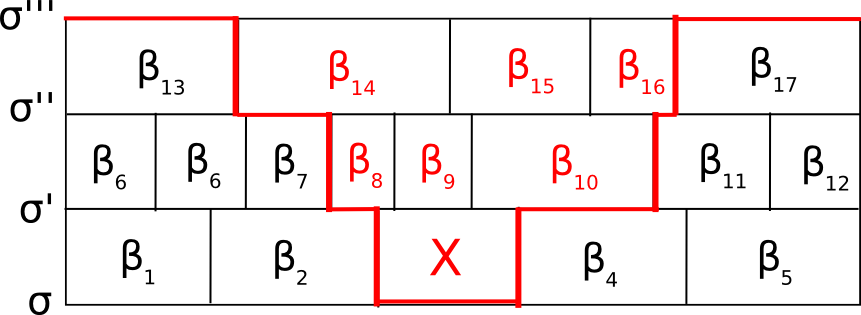
\includegraphics[width=200pt]{revert3.png}
\end{center}

Notice that one can apply the set of still-valid blocks sequentially to $\sigma$ to obtain $\sigma'_f$ in all cases.
\end{proof}

It is important to note that the revert process is scalable only if the number of subspaces that an attacker can revert with a single invalid block is bounded, assuming some bound on the amount of time that it takes for the bad block to be detected and for the revert to be included. Otherwise, the attacker can annoy all users by paying less than $b * L$ cost, and so the algorithm will no longer be scalable under attack. In order to achieve this, we have two solutions. First, we can specify that each block can have a maximum area size $k$ for some fixed $k$. The other approach is to require blocks with area larger than $k$ subspaces to have proportionately more validators; \eg a block with area of size $4k$ subspaces should require $\frac{8m}{3}$ signatures out of a pool of $4m$ in order to be valid. Both strategies ensure scalability under attack.

\section{Stacking}

The above schemes provide scalability up to $O(N^{2-\epsilon})$. But can we go higher than that? As it turns out, the answer is yes; we can in fact achieve scalability of $O(N^{d-\epsilon})$ for arbitrary $d$ while satisfying both economic and Byzantine-fault-tolerance guarantees. We accomplish this by essentially layering the scheme on top of itself. We replace the two-level system with a generalized system with $d$ levels: the header chain, level 1 collations, level 2 collations ... level $d-1$ collations and then finally transactions. Each level $i$ collation contains $n$ level $i+1$ collations, except the level $d-1$ collations which contain transactions. We create a $d$-tiered partitioning scheme, where the state is partitioning into $n$ level 1 subspaces, then each level $i$ subspace is partitioned into $n$ level $i+1$ subspaces, stacking $d$ times where the final level is accounts.

\begin{center}
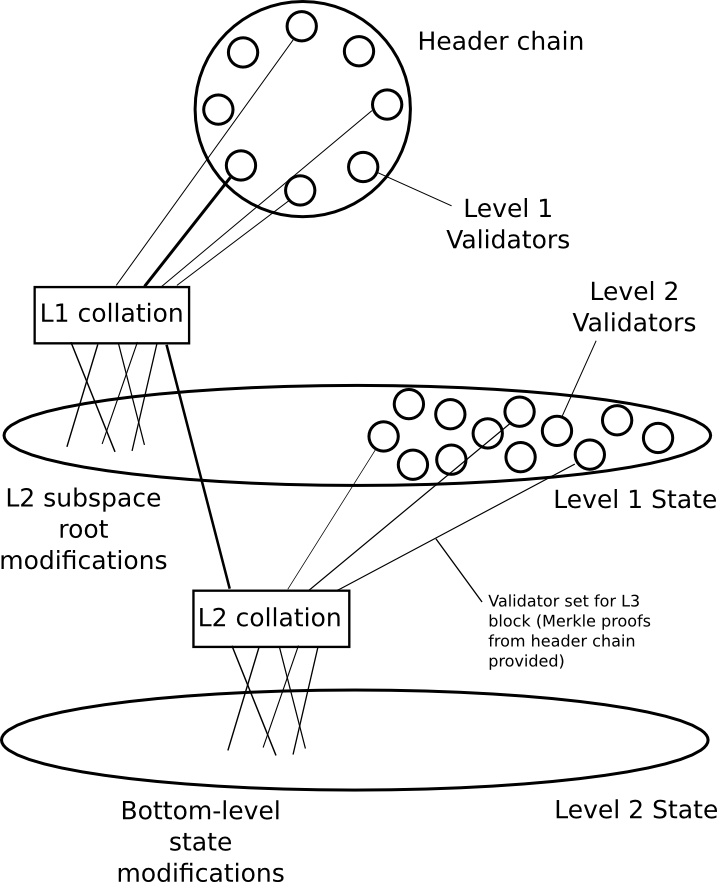
\includegraphics[width=250pt]{multilevel.png}
\end{center}

Each level $i$ collation includes $AP$ and $AN$ values as before, calculating $AN$ by determining the root of each level $i$ subspace in the new area, except that the root is calculated using the level $i+1$ collations included in the level $i$ collation. The validity of a level $i$ collation for $i < d-1$ is defined narrowly, just as is the validity of a header chain, and does not include the validity of transactions or level $i+2$ collations contained in that collation; all that matters is that the headers of the level $i+1$ collations are available that the $AP$ values are calculated correctly. If a level $i+1$ collation inside of a level $i$ collation turns out to be invalid, that is handled through the purgatory and revert process inside of level $i$.

There are also now multiple pools of validators, one for each level: level $1$ validators in the header chain, level $2$ validators in the level 1 subspace, etc. A collation on level $i$ must be approved by a random selection of $m$ level $i$ validators. Given that the set of validators at any level may change during a block, we clarify that we are concerned with validators \emph{at the end of the previous block}; this removes concerns that, because validators are now not in the header chain and thus require Merkle proofs, they need to be included in some kind of observed area. Additionally, we add a rule that if a particular level $i$ collation is challenged and requires more than $O(N)$ validators to rescue it, we instead require it to be rescued by a pool of $m$ level $i-1$ validators (and if more than $O(N^2)$ validators are required, then $m$ level $i-2$ validators, and so on); this keeps the size of rescue operations, as well as the random choice lottery, to below $O(N)$. 

Suppose that the scheme is attacked, by means of a successful invalid level $i$ collation. Then, challenges would be placed at depth $i$, and eventually the collation's time in purgatory would expire and the revert procedure would happen, reverting the $i$-th level subspace roots. The reversion process would itself require an object at depth $i$ in order to process. Because the total economic volume is $O(N^{d-\epsilon})$, and there are $O(N^{i-\epsilon})$ validators at depth $i$, the cost of bribing $m$ validators at depth $i$ would be $m * N^{d - i}$, and the block would inconvenience roughly $O(N^{d - i})$ users, so a proportionality of attacker cost to network cost is maintained. The same escalation argument as before shows that the scheme does not become unscalable until the attacker starts making economic sacrifices superlinear in the economic activity in the blockchain.

In practice, we expect that the extra complexity in implementing such an ultra-scalable scheme will be sufficiently high that cryptoeconomic state machine developers will stick to simpler two-level scaling models for some time. However, the result is important as it shows that, fundamentally, the level of overhead required in order to have a blockchain of size $L$ is roughly $m * log(L)$, a very slowly-growing value. With clever use of zk-SNARKs, perhaps even a completely constant-overhead approach for blockchains of arbitrary size can be achieved.

\section{Strategy}

The above sections described the \emph{algorithms} that can be used to convert a state transition function into validity criteria that can be used in order to build a scalable blockchain architecture out of traditional non-scalable components. However, there is also a need to develop higher-level \emph{strategies} that would be used by validators in order to allow a maximally expressive set of state transitions to effectively execute.

One major category of strategy that must be developed is for \emph{index selection}. Each collator must determine what set of subspace indices they will be keeping up to date on the state for, and be willing to produce collations containing. In the event that transactions requiring a larger area appear, the groups of collators will likely need to somehow cooperate in order to be able to produce a collation containing the combined area. One possible strategy is for validators to arrange subspace indices in a k-dimensional space, and maintain up-to-date knowledge of $\sigma[i]$ for either a radius-r cube or at least two adjacent subspaces. An alternative approach, specialized to simpler state transition functions involving sending from A to B (such as that of Bitcoin), is to maintain $(i, j)$ pairs and update $i$ and $j$ often. A third approach is adaptive: use some kind of algorithm to determine which subspace indices appear together most often, and try to keep track of an increasingly contiguous cluster over time. If transaction senders also adapt their activities to subspace boundaries, the co-adaptation process can potentially over time create highly efficient separations.

Additionally, note that index selection also becomes a concern when one or more collations is in purgatory. In this case, a collation producer producing a collation on top of a collation in purgatory has the concern that their collation may be reverted. Hence, a possible strategy that collators may employ in that case is to compute the dependency cones of all presently challenged collations, and refuse to produce collations that are fully or partially inside any such dependency cone. In that case, however, the collation producer may also wish to check availability on the contested collation themselves, and if it is contested create a rescue object.

The other category of strategy is for transaction sending, particularly in the context of more complex state transition functions like that used in Ethereum. If a transaction only affects a few neighboring subspaces, then an index selection strategy as above will be able to provide easy and global transfer. However, what happens if an action needs to be performed that has wide-reaching effect, and it is impractical to put it into a single collation? In this case, one option is to set up an ``asynchronous routing'' meta-protocol: if a transaction affects state $\sigma[i]$ but also needs to effect a change in $\sigma[j]$, then if it is acceptable for the latter change to be asynchronous we can have a message be passed through a ``network'' of contracts, first to a contract in a state neighboring $\sigma[i]$, then hopping progressively closer to $\sigma[j]$ during subsequent transaction executions until finally arriving at $\sigma[j]$ and effecting the desired change. Note that this is equivalent to the hypercubes \cite{hypercubes} strategy developed for Ethereum in 2014; but instead of being a core part of the protocol, the protocol has been abstracted even further out allowing hypercubes to simply be one of the many possible strategies that the protocol can lead to.

If the primary purpose of a blockchain is to act as a currency system, then as long as sufficient liquidity exists one can get by with a very low amount of interoperability. For example, even if it is only possible to move funds between subspaces every 1000 blocks, and even then only through a single central ``hub state'' (which is assumed all nodes store as a strategy), that limited movement provides enough fungibility for the currency units in the various subspaces to maintain fungibility. Cross-subspace payments can be done by means of various decentralized exchange protocols, treating the different subspaces as different currencies with the only difference being that the currency exchange rate will always remain equal to 1. However, it is debatable whether this approach is preferable to the other strategy described above of having collators select random $(i, j)$ pairs.

Finally, there is the protocol-level decision of how to maintain the divisions between subspaces and grow and shrink the total number of subspaces if necessary. There are several categories of solution here:

\begin{itemize}
\item
Employ an adaptive algorithms, perhaps adapting Karger's minimal-cut algorithm \cite{karger}, in order to split and join subspaces over time. Note that this can be done at the strategy level, giving the top-level consensus the right to split and join subspaces arbitrarily, but making it economically efficient for them to make splits that create a minimal cut. One disadvantage of this approach is that if transaction fees are priced so as to disincentivize cross-subspace activity, fees for specific operations become unpredictable since subspaces can be rearranged.
\item
Create new subspaces every time existing subspaces get too large, and incentivize users that marginally care less about network effect to act in those subspaces by lowering transaction fee pricing. This removes the ability to make arbitrary splits, but also leads to unpredictable pricing since prices do need to go up to incentivize users away from high-activity subspaces - although the pricing would be far more even and less discretionary.
\item
Allow users to set the location of objects in the state with arbitrary fineness, but with increased cost for higher degrees of fineness. Hence, objects that need to be very close to each other can pay the cost for extreme co-location, whereas other objects can place themselves further apart. This is the strategy undertaken in Gavin Wood's fiber-chains proposal\cite{fiberchains}.
\end{itemize}

\section{Further optimizations}

The algorithms described above are meant to be starting points, and are by no means optimal. The primary areas of optimization are likely to be the following:

\begin{itemize}
\item
Reducing the limits imposed on state transition functions while maintaining identical levels of scalability
\item
Achieving constant-factor gains by increasing efficiency of Merkle proofs, block sending protocols, safely reducing the value of $m$, reducing churn, etc.
\item
Increasing block speed
\item
Making reverts less harmful by using inclusive blockchain protocols (\ie if $\beta_1 ... \beta_n$ is the set of blocks that was reverted, and $\sigma'_f$ is the post-revert state, automatically update to $\sigma''_f$ = $\sigma'_f {++} \beta_1 {++} ... {++} \beta_n$).
\item
Providing the option for even higher gains of efficiency but at the cost of less-than-perfect guarantees of atomicity, \ie reducing $m$ to $8$ with the associated cost gains but with the understanding that the action happens within a cordoned-off area of the state where invalid transitions will sometimes happen.
\item
Reducing the number of signature verifications required at the top level (while keeping the number of validators per collation) constant.
\end{itemize}

For the first of these, the most promising direction where one can find easy immediate gains is to try to separate observed area from affected area. Theoretically, there is no interference risk if two collations in a block share observed areas, as long as that observed area is not any collation's affected area. The challenge is (i) figuring out what hard limits to impose on a collation in order to make sure that the scheme remains scalable (\eg if there are $\frac{n}{2}$ blocks each using $\{\frac{n}{2}+i\}$ as their observed area and $[\frac{n}{2}]$ as their observed area, the super-block will have $\frac{n^2}{4}$ hashes and will thus be unscalable), and (ii) figuring out how to manage reverts.

If one wants to go even further, one can allow the affected area of one collation to be the observed area of another collation, as long as one can arrange all collations in an order such that each collation is observed before it is affected. But there is a fundamental tradeoff between expressivity and fragility: the more the state transition function is able to process synchronous updates of very many and arbitrary states, the more costly a successful attack becomes if it must be reverted.

For the second, the largest tradeoff is likely to be that between churn and security. If one can keep the same $m$ nodes validating the same subspaces for a longer period of time, \eg half an hour, one may be able to reduce network load. Collators may even find it worth their while to download the entire upper half or two thirds of the Merkle tree for the subspaces into which they are sorted, allowing for 2x or 3x savings in the data that needs to be transmitted at the cost of $O(N^{0.5})$ or $O(N^{0.67})$ additional bandwidth per half hour (\eg assuming a subspace is 1 GB, either 32 KB or 1 MB per half hour, respectively). However, keeping a constant pool for too long makes the scheme more attackable.

For the third, the most likely source of gains will be a combination of two factors. First, the underlying non-scalable consensus algorithm can be sped up, using inclusive blockchain protocols such as those developed by Sompolinsky and Zohar\cite{inclusive} or proof-of-stake-based alternatives. Second, we can amend the top-level validity rule to say that collations do not need signatures in order to enter the header chain; however, in order for a state root to be considered finalized it must be signed and the signature must enter the header chain after the fact. This allows collations to be ``partially confirmed'' and even allows collations to be built on top of partially confirmed collations, as long as everything is fully confirmed eventually. Efficiency in such a scheme can be increased further, as a single validator signature can be used to attest to multiple collations by using an identifier.

For the fifth, an ideal goal would be to have a blockchain design which allows users to pick a point on the entire tradeoff space between cost and probability of failure, essentially capturing in the base protocol concepts like ``auditable computation'' \cite{auditable} (where computation is done by a third party by default, but if an auditor finds the third party provided an incorrect result the auditor can force the execution to be re-done on the blockchain and if the third party is indeed in the wrong it loses a security deposit from which the auditor will be able to claim a bounty).

For the sixth, the simplest strategy is to separate \emph{collation inclusion} from \emph{collation verification}. We can do this by allowing collations to enter the header chain unsigned, but first placing them in a special ``pending'' status. Validators can then sign collations on the header chain, and once a collation has been signed enough times it becomes accepted pending challenges and starts counting down the timer until finalization. The benefit here is that a single signature can be used to attest to the validity of multiple collations, by having the validator sign an encoded list of indices of collations that they believe are valid.

Finally, there is plenty of room for optimization in strategies, figuring out how validators can self-organize in order to maximize the expressivity of the state transition function in practice. The ideal goal is to present an interface to developers that ``just works'', providing a set of highly robust abstractions that achieve strong security bounds, freeing developers of the need to think about the underlying architecture, math and economics of the platform unless absolutely necessary. But this problem can be solved much later than the others, and solutions can much more easily continue to be iterated even after the underlying blockchain protocol is developed.

\section{Conclusion}

Using the reference-by-state-root homomorphism scheme described here, we can create blockchain protocols with the ability to process $O(N^{2-\epsilon})$ transactions in an environment where no user has access to more than $O(N)$ computational power. The scheme that we describe has the particular benefit that it makes very few assumptions about the underlying state transition function, except that it includes a currency which can be used to hold security deposits, and it makes very few assumptions about the underlying consensus algorithm, except that there exists some concept of a ``block maker'' (\emph{proposer} in Tendermint, \emph{miner} in Bitcoin) - and even that requirement can be dispensed with if we are not interested in economic security.

The scheme makes minimal compromises to security, scalability or interoperability, except for making the compromise that state transitions must be localized to a small area with a high degree of correlation between the subspaces that are modified together. In those cases where rare combinations of subspaces must be modified by one transaction, we offer the second-best alternative of asynchronicity via a hypercube-style relay network. Although one may criticize the solution for adding a higher amount of complexity at the bottom layer, we argue that this brings a tradeoff of significantly reducing complexity for application developers, who are exposed to an interface almost unchanged from non-scalable blockchains; developers have no additional need to think about cryptoeconomic security margins, trusted parties or rigging up application-specific revert procedures to ensure cross-chain atomic transactions. We hope that the higher throughput and lower transaction fees that will result from our designs can form the basis for a next wave of blockchain adoption.

\begin{thebibliography}{34}

\bibitem{mmpetertodd}
    Peter Todd on merge-mining, Dec 2013: \url{http://sourceforge.net/p/bitcoin/mailman/message/31796158/}

\bibitem{coiledcoin}
    What is the story behind the attack on CoiledCoin? (StackExchange, 2013): \url{http://bitcoin.stackexchange.com/questions/3472/what-is-the-story-behind-the-attack-on-coiledcoin}

\bibitem{factompetertodd}
    Peter Todd on Factom and checkpointing, Bitcoin subreddit: \url{https://www.reddit.com/r/Bitcoin/comments/2z9k5p/factom_announces_launch_date_for_software_token/cph0pvo?context=3}

\bibitem{parallelcomputing}
    Amdahl and Gustafson's laws and Bernstein's conditions for parallelizability (Wikipedia): \url{http://en.wikipedia.org/wiki/Parallel_computing#Amdahl.27s_law_and_Gustafson.27s_law}

\bibitem{gmaxwell}
    Gregory Maxwell and jl2012, Bitcointalk: \url{https://bitcointalk.org/index.php?topic=277389.45;wap2}

\bibitem{versum}
    VerSum: Verifiable Computations over Large Public Logs: \url{http://dl.acm.org/citation.cfm?id=2660327&dl=ACM&coll=DL}

\bibitem{lightning}
    Lightning Network: \url{http://lightning.network/}

\bibitem{tendermint}
    Tendermint: Consensus without mining, Jae Kwon: \url{http://tendermint.com/docs/tendermint.pdf}

\bibitem{stellar}
    Stellar Consensus Protocol, David Mazieres: \url{https://www.stellar.org/papers/stellar-consensus-protocol.pdf}

\bibitem{chenhouwu}
    Decentralized Consensus for P2P Network with Trust Relationships, Houwu Chen, \url{http://arxiv.org/abs/1501.06238}

\bibitem{zamfir}
    Vlad Zamfir's Formalizing Decentralized Consensus, coming soon.

\bibitem{piketty}
    Thomas Piketty, Capital in the 21st Century: \url{http://www.amazon.com/Capital-Twenty-First-Century-Thomas-Piketty/dp/1491534656}

\bibitem{bar}
    BAR Fault Tolerance for Cooperative Services, Amitanand S. Aiyer et al: \url{http://cs.brown.edu/courses/csci2950-g/papers/bar.pdf}

\bibitem{amiller}
    Anonymous Byzantine Consensus from Moderately-Hard Puzzles: A Model for Bitcoin, Andrew Miller, Joseph J LaViola Jr: \url{https://socrates1024.s3.amazonaws.com/consensus.pdf}

\bibitem{merkle}
    Merkle trees (Wikipedia): \url{http://en.wikipedia.org/wiki/Merkle_tree}

\bibitem{mpt}
    Merkle-Patricia trees (Ethereum): \url{https://github.com/ethereum/wiki/wiki/Patricia-Tree}

\bibitem{kademlia}
    Kademlia: A Peer-to-peer Information System Based on the XOR Metric \url{http://pdos.csail.mit.edu/~petar/papers/maymounkov-kademlia-lncs.pdf}

\bibitem{ipfs}
    IPFS: \url{http://ipfs.io/}

\bibitem{nxtinside}
    nxtinside.org, describing the NXT generation signature algorithm: \url{http://nxtinside.org/inside-a-proof-of-stake-cryptocurrency-2/}

\bibitem{snark}
    Succinct Zero-Knowledge for a von Neumann Architecture, Eli ben Sasson et al, Aug 2014: \url{https://eprint.iacr.org/2013/879.pdf}

\bibitem{schellingcoin}
    SchellingCoin: A Zero-Trust Universal Data Feed, Vitalik Buterin, Mar 2014: \url{https://blog.ethereum.org/2014/03/28/schellingcoin-a-minimal-trust-universal-data-feed/}

\bibitem{pepsilon}
    The P + Epsilon Attack, Vitalik Buterin, Jan 2015: \url{https://blog.ethereum.org/2015/01/28/p-epsilon-attack/}

\bibitem{sztorc}
    Truthcoin: Trustless, Decentralized, Censorship-Proof, Incentive-Compatible, Scalable Cryptocurrency Prediction Marketplace, Paul Sztorc, Aug 2014: \url{http://www.truthcoin.info/papers/truthcoin-whitepaper.pdf}

\bibitem{sztorc2}
    New attack that the consensus might be vulnerable to, Truthcoin forum, Paul Sztorc: \url{http://forum.truthcoin.info/index.php/topic,173.msg849.html#msg849}

\bibitem{swanson}
    Permissioned Distributed Ledger Systems, Tim Swanson: \url{http://www.ofnumbers.com/wp-content/uploads/2015/04/Permissioned-distributed-ledgers.pdf}

\bibitem{tomlion}
    1tf.org, discussion on the cryptoeconomic security margins of RANDAO, Vitalik Buterin and Tomlion: \url{http://1tf.org/bbs/index.php?p=/discussion/180/} (Chinese)

\bibitem{ntrusign}
    NTRUSign: Digital Signatures Using The NTRU Lattice, Jeffrey Hoffstein et al: \url{http://www.math.brown.edu/~jpipher/NTRUSign_RSA.pdf}

\bibitem{hashladder}
    Hash Ladders for Shorter Lamport Signatures, Karl Gluck: \url{https://gist.github.com/karlgluck/8412807}

\bibitem{sphincs}
    SPHINCS: Practical Stateless Hash-based Signatures, Daniel Bernstein et al: \url{http://sphincs.cr.yp.to/}

\bibitem{econofcrime}
    Economics of Crime, Erling Eide, Paul H Rubin, Joanna Mehlop Shepherd: \url{https://books.google.ca/books?id=gr95IhFHXHoC&pg=PA45}

\bibitem{treechains}
    Tree Chains, Peter Todd: \url{https://www.mail-archive.com/bitcoin-development@lists.sourceforge.net/msg04388.html}

\bibitem{laplace}
    Laplacian succession: \url{http://understandinguncertainty.org/node/225}

\bibitem{hypercubes}
    Scalability, Part 2: Hypercubes, Vitalik Buterin, October 2014: \url{http://www.reddit.com/r/ethereum/comments/2jvv5d/ethereum_blog_scalability_part_2_hypercubes/}

\bibitem{karger}
    Karger's minimal-cut algorithm, Wikipedia: \url{http://en.wikipedia.org/wiki/Karger%27s_algorithm}

\bibitem{inclusive}
    Inclusive Blockchain Protocols, Yoad Lewenberg, Yonatan Sompolinsky, Aviv Zohar: \url{http://fc15.ifca.ai/preproceedings/paper_101.pdf}

\bibitem{fiberchains}
    Blockchain Scalability: Chain Fibers Redux: \url{https://blog.ethereum.org/2015/04/05/blockchain-scalability-chain-fibers-redux/}

\bibitem{auditable}
    Scalability, Part 1: Building on Top (incl Auditable Computation): \url{https://blog.ethereum.org/2014/09/17/scalability-part-1-building-top/}

\end{thebibliography}

\end{document}
